% ============================================================
%  main.tex  - Software Architecture Report (MLOps)
%  RULE: Only member A (nhom truong) may edit this file.
%        Every other member edits only their own section file.
% ============================================================

\documentclass[twoside,final]{hcmut-report}
\usepackage{codespace}

% -- Encodings ------------------------------------------------
\usepackage{gensymb,textcomp}

% -- Tables ---------------------------------------------------
\usepackage[table]{xcolor}
\usepackage{array,longtable,multicol,multirow,siunitx,tabularx}
\newcolumntype{L}[1]{>{\raggedright\arraybackslash}p{#1}}

% -- Diagrams -------------------------------------------------
\usepackage{tikz}
\usetikzlibrary{arrows.meta,positioning,shapes.geometric,fit}

% -- Lists ----------------------------------------------------
\usepackage{enumitem}

% -- Figures --------------------------------------------------
\usepackage{caption,float}
\usepackage[export]{adjustbox}
\graphicspath{{figures/}}

% -- References -----------------------------------------------
% Use \Cref{} instead of \ref{}
\usepackage[nameinlink]{cleveref}

% -- Hyperlinks -----------------------------------------------
\usepackage{url}

% -- Counter depth --------------------------------------------
\AtBeginDocument{\counterwithin{lstlisting}{section}}

% ============================================================
%  Document metadata - edit here to update the cover page
% ============================================================
\coursename{Software Architecture}
\reporttype{Final Report}
\title{MLOps Architecture: Design, Rationale, and Layered Model}
\advisor{& [Advisor name] &}
\stuname{%
  & Member A (Nhom truong) & XXXXXXX \\
  & Member B               & XXXXXXX \\
  & Member C               & XXXXXXX \\
  & Member D               & XXXXXXX \\
  & Member E               & XXXXXXX \\
  & Member F               & XXXXXXX \\
  & Member G (Ky thuat)    & XXXXXXX \\
}

% ============================================================
\begin{document}

\coverpage%

% -- Member list ----------------------------------------------
\section*{Member List \& Workload}
\newcounter{memberrowno}
\setcounter{memberrowno}{0}
\begin{center}
  \begin{tabular}{>{\stepcounter{memberrowno}\thememberrowno}llcc}
    \toprule
    \multicolumn{1}{c}{\textbf{No.}} & \textbf{Full name} & \textbf{Student ID} & \textbf{Contribution} \\
    \midrule
      & Member A (Nhom truong) & XXXXXXX & 100\% \\
      & Member B               & XXXXXXX & 100\% \\
      & Member C               & XXXXXXX & 100\% \\
      & Member D               & XXXXXXX & 100\% \\
      & Member E               & XXXXXXX & 100\% \\
      & Member F               & XXXXXXX & 100\% \\
      & Member G (Ky thuat)    & XXXXXXX & 100\% \\
    \bottomrule
  \end{tabular}
\end{center}
\clearpage

% -- Table of contents ----------------------------------------
\tableofcontents
\listoffigures
\listoftables
\clearpage

% ============================================================
%  Sections - each member owns exactly one file below
% ============================================================
% =====================================================================
% sections/01-introduction.tex  --  Member A
% Labels used by other sections: sec:introduction
% Cross-references to other members' sections (labels agreed by team):
%   sec:mlops-concepts, sec:michelangelo-overview (A)
%   sec:design-rationale (B), sec:pros-cons (C),
%   sec:layered-architecture (D), sec:conclusion (A)
% =====================================================================

\section{Introduction}
\label{sec:introduction}

Machine learning (ML) has moved from a research activity to a core
component of production software, yet the engineering effort required to
operate ML systems is routinely underestimated. Sculley et al.\ observe
that developing and deploying ML systems is relatively fast and cheap,
whereas maintaining them over time is difficult and expensive, because
ML systems inherit all the maintenance problems of conventional code and
add a set of ML-specific ones, such as data dependencies, feedback loops
and sensitivity to changes in the external world~\cite{sculley2015hidden}.
In a typical real-world ML system, the model code is only a small part;
most of the system consists of surrounding infrastructure for data
collection, feature extraction, serving and monitoring~\cite{sculley2015hidden}.
Empirical studies confirm that the ML workflow is data-centric and highly
non-linear, with frequent feedback loops between data, modelling and
deployment stages~\cite{amershi2019software}. \emph{Machine Learning
Operations} (MLOps) has emerged as the engineering paradigm that addresses
this gap by combining ML, software engineering (in particular DevOps) and
data engineering to bring ML products into production and keep them
there~\cite{kreuzberger2023mlops}.

This report studies MLOps through the lens of \emph{software architecture},
using Uber's internal ML platform \emph{Michelangelo} as a case study.
Before Michelangelo, data scientists at Uber built models with a
heterogeneous set of tools, while engineering teams built bespoke,
one-off systems to run those models in production; there was no
standard way to store and compare experiments and no established path
to deployment~\cite{delbalso2017meet}. Michelangelo was created to
standardise this end-to-end workflow~\cite{delbalso2017meet} and has
since evolved through three phases: predictive ML on tabular data,
deep learning (DL), and generative AI~\cite{wang2024predictive}. We
select Michelangelo for three reasons. First, it is one of the earliest
documented enterprise ML platforms, and its feature store is described
by authors involved in building it as the first industrial feature
store~\cite{orr2021managing}. Second, its design and evolution are
documented both in peer-reviewed publications~\cite{li2017scaling,sun2020gallery}
and in a series of engineering reports spanning eight
years~\cite{delbalso2017meet,delbalso2018scaling,wang2024predictive},
including Uber's own account of mistakes and lessons learned. Third, it
operates at a scale that makes architectural trade-offs visible: as of
2024, the platform manages about 400 active ML projects, runs more than
20{,}000 training jobs per month, and hosts over 5{,}000 production models
that serve up to 10 million real-time predictions per second at
peak~\cite{wang2024predictive}.

The report addresses four questions: (i)~which MLOps concepts a platform
such as Michelangelo must realise; (ii)~why Michelangelo was designed the
way it is; (iii)~what trade-offs this design entails; and (iv)~how its
layered architecture organises the platform's responsibilities.
Section~\ref{sec:mlops-concepts} defines the core MLOps concepts and maps
each to its Michelangelo counterpart, and
Section~\ref{sec:michelangelo-overview} summarises the platform's evolution
from 2015 to 2024 together with its six-step workflow.
Section~\ref{sec:design-rationale} derives the main design decisions from
the problems Uber faced in 2015. Section~\ref{sec:pros-cons} discusses
the platform's strengths, weaknesses and trade-offs, including a brief
comparison with alternative platforms. Section~\ref{sec:layered-architecture}
analyses Michelangelo as a layered architecture, and
Section~\ref{sec:conclusion} concludes the report.
% TODO (A): adjust the sentence above if B/C/D change the scope of their sections.
% TODO (A): if G's demo is described in the report, add one sentence here
%           and a \ref to the corresponding section/appendix.          % Member B
% =====================================================================
% sections/02-mlops-concepts.tex  --  Member A
% Contains two sections:
%   \section{MLOps Concepts}            \label{sec:mlops-concepts}
%   \section{Overview of Michelangelo}  \label{sec:michelangelo-overview}
% Required packages in main.tex: booktabs, graphicx, amsmath (or amssymb)
% Figure: figures/michelangelo-workflow.pdf (fig:workflow)
% =====================================================================

\section{MLOps Concepts}
\label{sec:mlops-concepts}

Kreuzberger et al.\ define MLOps as a paradigm, comprising best practices,
concepts and a development culture, for the end-to-end conceptualisation,
implementation, monitoring, deployment and scalability of ML products; it
aims to productionise ML systems by bridging development and
operations~\cite{kreuzberger2023mlops}. Their study identifies nine
principles, including CI/CD automation, versioning, continuous training,
metadata tracking and continuous monitoring, which are realised by
technical components such as a feature store, a model registry and a
monitoring component~\cite{kreuzberger2023mlops}. This section introduces
the six concepts used throughout the report. For each concept we give a
definition from the literature and its counterpart in Michelangelo;
Table~\ref{tab:concept-mapping} summarises the mapping.

\subsection{ML Lifecycle}
\label{subsec:ml-lifecycle}

The \emph{ML lifecycle} is the sequence of activities required to build
and operate an ML model. Amershi et al.\ describe a nine-stage workflow
observed at Microsoft: model requirements, data collection, data
cleaning, data labelling, feature engineering, model training, model
evaluation, model deployment and model monitoring~\cite{amershi2019software}.
Unlike a conventional software process, this workflow is data-centric and
highly non-linear: evaluation and monitoring results frequently feed back
into earlier stages, for example when a distribution shift between
training and production data requires collecting new
data~\cite{amershi2019software}.
\textbf{In Michelangelo}, the lifecycle is condensed into a six-step
workflow (manage data, train, evaluate, deploy, predict, monitor) that
Uber reports to be shared by almost all of its ML use
cases~\cite{delbalso2017meet}. The platform is organised around this
workflow (Section~\ref{subsec:six-step-workflow}).

\subsection{CI/CD and Continuous Training}
\label{subsec:cicd-ct}

\emph{Continuous integration and continuous delivery/deployment} (CI/CD)
automate the build, test, delivery and deployment steps and give
developers rapid feedback~\cite{kreuzberger2023mlops}. ML adds a third
practice, \emph{continuous training} (CT): the periodic retraining of a
model on new feature data, enabled by a monitoring component, a feedback
loop and an automated workflow pipeline, and always accompanied by an
evaluation run that assesses the change in model
quality~\cite{kreuzberger2023mlops}.
\textbf{In Michelangelo}, early automation was exposed through an API:
many teams scheduled regular retraining and redeployment with their own
scripts, while others, such as the UberEATS delivery-time team, still
triggered both steps manually from the web UI~\cite{delbalso2017meet}.
Gallery added rule-based automation: user-defined rules over stored
performance metrics can detect model drift, raise alerts and trigger
retraining for an individual model, for example for a single city,
instead of retraining all models blindly~\cite{sun2020gallery}.
CI/CD became a platform capability with Project Canvas (2020), which
stores all ML code and configuration in a monorepo, packages training
and serving code into immutable Docker images, and automatically deploys
models merged into the main branch after tests and
validations~\cite{wang2024predictive}. The unified MA Studio interface
adds incremental zonal rollout with automatic rollback triggers to
deployment~\cite{wang2024predictive}.

\subsection{Feature Store}
\label{subsec:feature-store}

A \emph{feature store} provides central storage for commonly used
features and typically combines an offline store, which serves features
with normal latency for experimentation and training, with an online
store, which serves features with low latency for production
inference~\cite{kreuzberger2023mlops}. Feature stores emerged to avoid
duplicated feature engineering across teams and inconsistent feature
definitions, and to keep deployed models supplied with fresh
features~\cite{orr2021managing}.
\textbf{In Michelangelo}, the feature store (later named
\emph{Palette}) uses Hive as the offline store and Cassandra as the
online store; features are computed by Spark batch jobs or by Samza
streaming jobs~\cite{li2017scaling}. A model refers to a feature only by
its canonical name, and the platform resolves the name to the correct
offline or online source~\cite{delbalso2017meet}. Uber reports freshness
guarantees of under 12 hours for historical features and under 5 minutes
for near-real-time features, each served with about 10\,ms query
latency~\cite{li2017scaling}. The store grew from approximately 10{,}000
features in 2017~\cite{delbalso2017meet} to more than 20{,}000 in
2024~\cite{wang2024predictive}.

\subsection{Model Registry}
\label{subsec:model-registry}

A \emph{model registry} centrally stores trained models together with
their metadata, such as training parameters, performance metrics and
lineage, to support reproducibility and versioning~\cite{kreuzberger2023mlops}.
Open-source platforms such as MLflow address the same need for tracking
experiments and packaging models for deployment~\cite{zaharia2018accelerating}.
\textbf{In Michelangelo}, every trained model is stored as a versioned
object that records, among other things, who trained it, its full
configuration, references to the training and test data, feature
importance, accuracy metrics and the learned
parameters~\cite{delbalso2017meet}. At serving time, a client addresses a
model either by its UUID or by a tag; deploying a new model with the same
signature to an existing tag switches traffic to it without any change to
client code~\cite{delbalso2017meet}.

The registry role was later consolidated in \emph{Gallery}, a model
lifecycle management system originally built by Uber's Marketplace
Forecasting team and subsequently integrated into
Michelangelo~\cite{sun2020gallery}. Before Gallery, Uber engineers used
more than seven different storage solutions to save models, including
MySQL, HDFS, Cassandra and Git repositories~\cite{sun2020gallery}. Gallery
is designed around four principles: models are \emph{immutable}, so every
update creates a new version; the system is \emph{model-neutral} and
\emph{framework-agnostic}, storing trained models as uninterpreted binary
blobs; and lifecycle transitions are \emph{automated}~\cite{sun2020gallery}.
It distinguishes a \emph{model} (the specification of a transformation,
such as features and hyper-parameters) from a \emph{model instance} (the
parameters learned from a particular training set), assigns each instance
a Git-style UUID linked to a base version, and tracks dependencies
between models whose outputs feed one another~\cite{sun2020gallery}.
Metadata and metrics are kept in a relational database for search, while
model blobs reside in distributed storage~\cite{sun2020gallery}. A rule
engine evaluates user-defined, peer-reviewed rules over these metrics,
either to select a \emph{champion} model for serving or to trigger actions
such as deployment~\cite{sun2020gallery}. As part of Michelangelo, Gallery
manages more than one million model instances, and for Uber's forecasting
models it reduced deployment effort from two hours of engineering work
per model to none~\cite{sun2020gallery}. Our demonstrator reproduces the
tag-based switching mechanism with MLflow model aliases.

\subsection{Training/Serving Skew}
\label{subsec:train-serve-skew}

\emph{Training/serving skew} is a discrepancy between the data used to
train a model and the data it receives in production. Breck et al.\
identify the use of different code paths to generate training and
serving data as its most common cause, and distinguish three forms:
\emph{feature skew} (a feature takes different values at training and
serving time), \emph{distribution skew} (the feature distribution in
training differs from that at serving time) and \emph{scoring/serving
skew} (only a subset of scored examples is actually served, which biases
future training data)~\cite{breck2019data}.
\textbf{In Michelangelo}, the primary safeguard is a single code path:
each feature is computed by one pipeline for both training and
prediction~\cite{li2017scaling}, and feature selection and transformation
are expressed in a domain-specific language (DSL) whose expressions are
stored in the model configuration and applied identically at training
and prediction time~\cite{delbalso2017meet}. In Michelangelo~2.0, the
transformations are bundled with the model, including DL-native
transformations compiled into the inference graph, and MA Studio provides
an online/offline feature consistency check~\cite{wang2024predictive}.
At the model level, Gallery stores training, validation and production
metrics for every model instance, so that \emph{production skew}, a gap
between training-time and serving-time performance, can be
detected~\cite{sun2020gallery}.

\subsection{Monitoring and Drift}
\label{subsec:monitoring-drift}

Because the external world is rarely stable, live monitoring combined
with automated response is critical for the long-term reliability of ML
systems~\cite{sculley2015hidden}. A principal reason is \emph{concept
drift}, formally a change in the joint distribution of inputs $X$ and
target $y$ between two points in time~\cite{gama2014survey}:
\begin{equation}
  \exists X : p_{t_0}(X, y) \neq p_{t_1}(X, y).
  \label{eq:concept-drift}
\end{equation}
Gama et al.\ distinguish \emph{real} concept drift, a change in
$p(y \mid X)$ that affects predictive decisions, from \emph{virtual}
drift, a change in the input distribution $p(X)$ that does not affect
$p(y \mid X)$~\cite{gama2014survey}. Continuous monitoring therefore
covers data, model and serving performance~\cite{kreuzberger2023mlops}.
\textbf{In Michelangelo}, two complementary approaches are used. When
outcomes are observable, the platform logs predictions, joins them with
the observed labels and publishes accuracy metrics (e.g., RMSE and MAE)
to Uber's time-series monitoring system with threshold
alerts~\cite{delbalso2017meet,li2017scaling}. When labels are delayed or
unavailable, it compares the distributions of features and predictions
over time, which is less precise but still detects problematic
shifts~\cite{delbalso2018scaling}. Since Michelangelo~2.0, a Model
Excellence Score (MES) tracks quality dimensions such as prediction
accuracy, model freshness and feature quality against SLA-style
targets~\cite{wang2024predictive}.

\begin{table}[t]
  \centering
  \caption{MLOps concepts and their realisation in Michelangelo.}
  \label{tab:concept-mapping}
  \small
  \begin{tabular}{@{}p{0.22\linewidth}p{0.72\linewidth}@{}}
    \toprule
    \textbf{Concept} & \textbf{Michelangelo realisation} \\
    \midrule
    ML lifecycle &
      Six-step workflow shared by most use cases~\cite{delbalso2017meet} \\
    CI/CD/CT &
      API-scheduled retraining~\cite{delbalso2017meet}; rule-triggered
      retraining in Gallery~\cite{sun2020gallery}; Canvas monorepo, ML CI/CD
      and immutable images~\cite{wang2024predictive} \\
    Feature store &
      Palette: Hive (offline) and Cassandra (online), canonical feature
      names~\cite{li2017scaling,delbalso2017meet} \\
    Model registry &
      Versioned model repository with UUID/tag addressing~\cite{delbalso2017meet};
      Gallery: immutable model instances, metadata search, rule-based
      champion selection~\cite{sun2020gallery} \\
    Training/serving skew &
      One feature code path; shared DSL; consistency
      check~\cite{li2017scaling,delbalso2017meet,wang2024predictive} \\
    Monitoring \& drift &
      Prediction--outcome joins; distribution monitoring;
      MES~\cite{delbalso2017meet,delbalso2018scaling,wang2024predictive} \\
    \bottomrule
  \end{tabular}
\end{table}

% ---------------------------------------------------------------------

\section{Overview of Michelangelo}
\label{sec:michelangelo-overview}

\subsection{Evolution from 2015 to 2024}
\label{subsec:evolution}

Uber began building Michelangelo in mid-2015~\cite{delbalso2017meet}, and
dates the first production version to 2016~\cite{wang2024predictive}.
Table~\ref{tab:timeline} summarises the three phases identified by
Uber~\cite{wang2024predictive}, each with representative metrics.

\emph{Michelangelo~1.0 (2016--2019)} targeted predictive ML on tabular
data, using algorithms such as XGBoost for ETA prediction, risk
assessment and pricing~\cite{wang2024predictive}. The initial focus was
large-scale batch training and batch prediction; a centralised feature
store, a low-latency real-time prediction service, DL workflows,
notebook integration and partitioned models were added
incrementally~\cite{delbalso2018scaling}.

\emph{Michelangelo~2.0 (2019--2023)} shifted the focus from enabling ML
everywhere to improving high-impact projects. It addressed four
shortcomings of version~1.0: the lack of a model-quality definition and
project tiering, insufficient DL support, poor support for collaborative
development, and fragmented tooling~\cite{wang2024predictive}. The
response included project tiering, model iteration as code via Canvas,
DL as a first-class citizen (Ray-based trainers and Triton-based
serving), and the unified MA Studio interface~\cite{wang2024predictive}.
Architecturally, the platform was reorganised into a control plane, an
offline data plane and an online data plane~\cite{wang2024predictive};
this structure is analysed in Section~\ref{sec:layered-architecture}.

\emph{Generative AI (2023--present)} extended the platform to LLMOps. A
Gen AI Gateway provides unified, policy-controlled access to external
and in-house large language models (LLMs), and the platform added a model
catalogue, an LLM evaluation framework, a prompt engineering toolkit, and
fine-tuning based on Hugging Face and DeepSpeed~\cite{wang2024predictive}.

\begin{table}[t]
  \centering
  \caption{Evolution of Michelangelo (phases as defined by Uber~\cite{wang2024predictive}).}
  \label{tab:timeline}
  \small
  \begin{tabular}{@{}p{0.17\linewidth}p{0.36\linewidth}p{0.39\linewidth}@{}}
    \toprule
    \textbf{Phase} & \textbf{Focus and key additions} & \textbf{Representative metrics} \\
    \midrule
    1.0 \newline (2016--2019) &
      Predictive ML on tabular data; feature store; real-time serving;
      partitioned models; Gallery; PyML; Horovod~\cite{delbalso2018scaling,wang2024predictive} &
      2017: $\approx$10{,}000 features; online P95 latency $<$10\,ms; top
      models $>$250{,}000 predictions/s~\cite{delbalso2017meet}.
      2018: thousands of production models; millions of predictions/s~\cite{delbalso2018scaling} \\
    \addlinespace
    2.0 \newline (2019--2023) &
      DL as first-class citizen; Canvas (2020); MA Studio; project
      tiering; Ray and Triton; three-plane architecture~\cite{wang2024predictive} &
      2020: $>$1\,M model instances managed by Gallery~\cite{sun2020gallery}.
      $>$5{,}000 GPUs; DL adoption in tier-1 projects from almost zero to
      $>$60\,\%~\cite{wang2024predictive} \\
    \addlinespace
    GenAI \newline (2023--) &
      Gen AI Gateway; LLM fine-tuning, evaluation and prompt
      management~\cite{wang2024predictive} &
      2024: $\approx$400 active projects; $>$20{,}000 training jobs/month;
      $>$5{,}000 production models; 10\,M predictions/s at peak~\cite{wang2024predictive} \\
    \bottomrule
  \end{tabular}
\end{table}

\subsection{The Six-Step Workflow}
\label{subsec:six-step-workflow}

Michelangelo was designed to provide scalable, reliable, reproducible
and automated tooling for a six-step workflow~\cite{delbalso2017meet},
illustrated in Figure~\ref{fig:workflow} and summarised below using
UberEATS estimated time of delivery (ETD) as the running example. The
ETD model is a gradient-boosted decision tree regressor whose features
combine request data, historical aggregates and near-real-time
aggregates~\cite{delbalso2017meet}.

\begin{enumerate}
  \item \textbf{Manage data.} Offline pipelines compute features from
    the HDFS data lake with Spark and Hive; online features are
    precomputed into Cassandra either by batch jobs or by Samza streaming
    jobs consuming Kafka~\cite{delbalso2017meet}. For ETD, a restaurant's
    average meal preparation time over the last seven days is a batch
    feature, whereas the same average over the last hour is a
    near-real-time feature~\cite{delbalso2017meet}.
  \item \textbf{Train models.} A model configuration specifies the
    model type, hyper-parameters, data source, feature DSL expressions
    and compute resources, and training runs as a distributed
    job~\cite{delbalso2017meet}. \emph{Partitioned models} train one model
    per node of a hierarchy (e.g., city and country) and fall back to the
    parent model when a partition lacks data; ETD is trained in this way
    as a single logical model for all cities~\cite{li2017scaling}.
  \item \textbf{Evaluate models.} Each trained model is stored in the
    model repository with accuracy reports, feature-importance reports and
    visualisations, enabling comparison across many candidate
    models~\cite{delbalso2017meet}.
  \item \textbf{Deploy models.} Models can be deployed offline (batch
    prediction in Spark jobs), online (a prediction service cluster
    called via RPC), or as an embedded library; model artifacts are
    distributed through Uber's standard code deployment
    infrastructure~\cite{delbalso2017meet}.
  \item \textbf{Make predictions.} The serving container applies the
    compiled DSL to raw features, fetches additional features from the
    feature store, and scores the final feature
    vector~\cite{delbalso2017meet}. Uber reports a 99th-percentile latency
    of 20\,ms for ETD serving under bursty meal-time
    traffic~\cite{li2017scaling}.
  \item \textbf{Monitor predictions.} Predictions are logged and joined
    with observed outcomes to compute live accuracy metrics and trigger
    alerts (Section~\ref{subsec:monitoring-drift}).
\end{enumerate}

\begin{figure}[t]
  \centering
  % Source files: figures/michelangelo-workflow.tex (TikZ),
  %               figures/michelangelo-workflow.drawio (editable copy for F).
  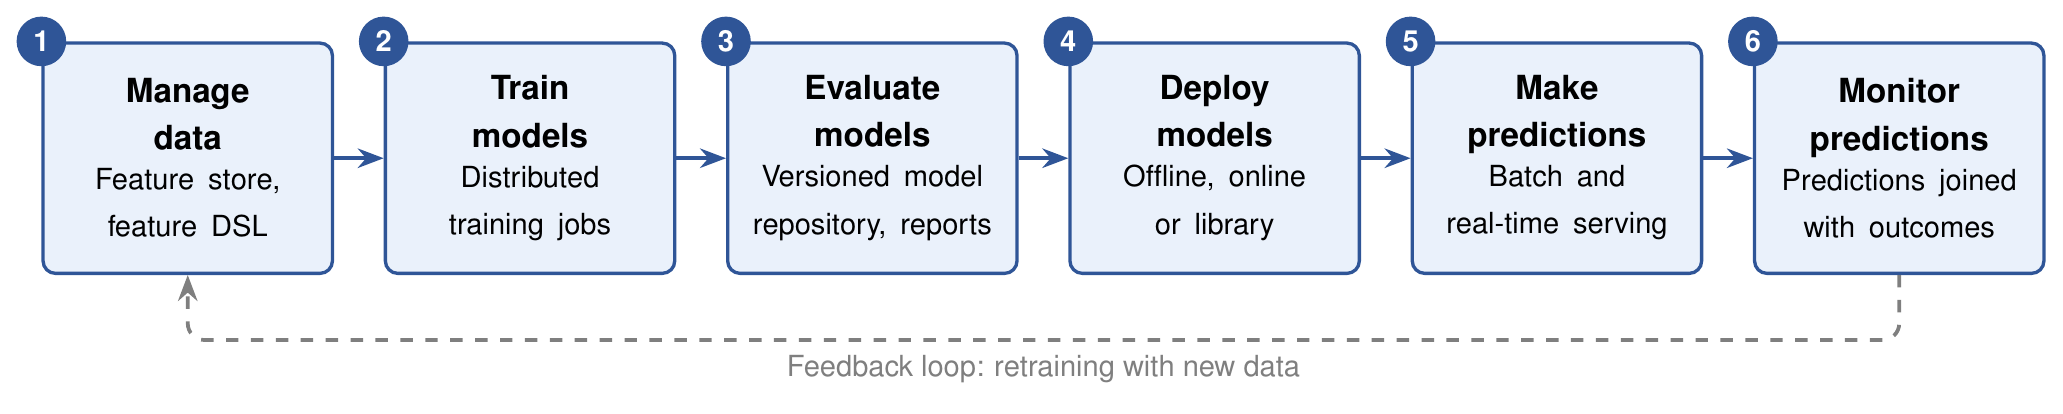
\includegraphics[width=\linewidth]{figures/michelangelo-workflow}
  \caption{Michelangelo's six-step ML workflow, based
    on~\cite{delbalso2017meet}. The dashed arrow denotes the feedback loop
    from monitoring back to data management and retraining.}
  \label{fig:workflow}
\end{figure}

A management plane, comprising a web UI, a REST API and a workflow
system, orchestrates data pipelines, training jobs, batch prediction and
model deployment across these steps~\cite{delbalso2017meet}. How this
plane and the data-processing components are layered, and how that
layering changed in Michelangelo~2.0, is the subject of
Section~\ref{sec:layered-architecture}.        % Member C
% sections/03-design-rationale.tex
% OWNER: Member B
% Do NOT edit this file if you are not Member B.
% Statements marked "our interpretation" are the authors' analysis, not claims made by Uber.

\section{Design Rationale}
\label{sec:design-rationale}

This section explains \emph{why} Michelangelo looks the way it does. It lists the
problems Uber faced when it started the platform (\Cref{sec:rationale-problems}),
traces each design decision back to those problems
(\Cref{sec:rationale-decisions}) and names the quality attributes the design
targets (\Cref{sec:rationale-qualities}). \emph{How} the resulting components are
arranged into layers is covered in \Cref{sec:layered-architecture}.

% ------------------------------------------------------------
\subsection{Uber's Problems in 2015}
\label{sec:rationale-problems}

Uber ``began building Michelangelo in mid 2015''~\cite{delbalso2017meet}. At that time ML
was ``not widely used at Uber'', and the company had ``no centralized ML efforts
and a few bespoke ML systems''~\cite{delbalso2018scaling}. The 2017 post names the concrete
gaps, which we number P1--P6 for use in the rest of this section:

\begin{enumerate}[label=\textbf{P\arabic*}]
  \item \label{prob:tools}\textbf{Fragmented tools.} Data scientists ``were
        using a wide variety of tools to create predictive models''~\cite{delbalso2017meet}.
  \item \label{prob:pipelines}\textbf{No reproducible pipelines.} There were
        ``no systems in place to build reliable, uniform, and reproducible
        pipelines''~\cite{delbalso2017meet}.
  \item \label{prob:desktop}\textbf{Desktop-sized training.} It was ``not
        possible to train models larger than what would fit on data scientists'
        desktop machines''~\cite{delbalso2017meet}.
  \item \label{prob:experiments}\textbf{No experiment tracking.} There was no
        ``standard place to store the results of training
        experiments''~\cite{delbalso2017meet}.
  \item \label{prob:deploy}\textbf{No standard deployment path.} There was ``no
        established path to deploying a model into production''. For each project,
        the engineering team ``had to create a custom serving container'', and
        separate teams built ``bespoke one-off systems'' to use models in
        production~\cite{delbalso2017meet}.
  \item \label{prob:features}\textbf{Duplicated feature work.} ``Many modeling
        problems at Uber use identical or similar features''~\cite{delbalso2017meet}.
        In addition, models deployed online ``cannot access data stored in
        HDFS''~\cite{delbalso2017meet}, so online models need another way to get their
        features at serving time.
\end{enumerate}

Uber's stated goal was to close these gaps ``by standardizing the workflows and
tools across teams'' and to ``create a system that would grow with the
business''~\cite{delbalso2017meet}.

% ------------------------------------------------------------
\subsection{From Requirements to Design Decisions}
\label{sec:rationale-decisions}

\Cref{tab:rationale} turns each problem into a requirement, the decision Uber made
to meet it and the component that implements the decision. The requirement
wording and the problem mapping in the last column are \emph{our
interpretation}; the decisions and components are taken from Uber's posts.

\begin{table}[ht]
  \centering
  \small
  \caption{Requirements, design decisions and components of Michelangelo.}
  \label{tab:rationale}
  \begin{tabularx}{\linewidth}{@{}L{2.6cm}>{\raggedright\arraybackslash}X L{2.8cm}L{1.3cm}@{}}
    \toprule
    \textbf{Requirement} & \textbf{Design decision} & \textbf{Component} & \textbf{Solves} \\
    \midrule
    Reuse features across teams
      & One shared, curated feature store; offline features in Hive tables on HDFS, online
        features precomputed into Cassandra~\cite{delbalso2017meet}
      & Feature store (later Palette)~\cite{delbalso2017meet,uber2024palette}
      & \ref{prob:features}, \ref{prob:tools} \\
    \addlinespace
    Same features in training and serving
      & A feature DSL whose ``same expressions are applied at training time and
        at prediction time''~\cite{delbalso2017meet}
      & Feature DSL, shared by training and serving~\cite{delbalso2017meet}
      & \ref{prob:pipelines}, \ref{prob:features} \\
    \addlinespace
    Train beyond one machine
      & Distributed training on Spark~\cite{delbalso2017meet}, later Horovod for
        deep learning~\cite{delbalso2018scaling} and Ray
        trainers~\cite{wang2024predictive}
      & Training jobs on Spark, Horovod,
        Ray~\cite{delbalso2017meet,delbalso2018scaling,wang2024predictive}
      & \ref{prob:desktop} \\
    \addlinespace
    Store and compare every experiment
      & Store each trained model as a versioned object with its configuration,
        learned parameters and evaluation report; compare models in the
        UI~\cite{delbalso2017meet}
      & Model repository~\cite{delbalso2017meet}, later Gallery~\cite{sun2020gallery}
      & \ref{prob:experiments}, \ref{prob:pipelines} \\
    \addlinespace
    One-click, safe deployment
      & Deploy through the UI or API; at serving time a model is found by
        ``its UUID and an optional tag (or alias)''~\cite{delbalso2017meet}
      & Model repository + deployment tags~\cite{delbalso2017meet}
      & \ref{prob:deploy} \\
    \addlinespace
    No custom serving per project
      & One shared prediction service that other services call over RPC,
        instead of a container per project~\cite{delbalso2017meet}
      & Online Prediction Service~\cite{delbalso2017meet,wang2024predictive}
      & \ref{prob:deploy}, \ref{prob:tools} \\
    \addlinespace
    One workflow for all teams
      & A single end-to-end platform with a web UI, API and workflow system over
        shared infrastructure~\cite{delbalso2017meet}
      & Michelangelo platform (API tier, UI)~\cite{delbalso2017meet}
      & \ref{prob:tools}, \ref{prob:pipelines} \\
    \bottomrule
  \end{tabularx}
\end{table}

\paragraph{Why these decisions.}
\begin{itemize}
  \item \textbf{A central feature store instead of per-team features.} Because
        many models use ``identical or similar features''~\cite{delbalso2017meet},
        computing a feature once and sharing it removes duplicate work
        (\ref{prob:features}). Uber later called the feature store ``critical to
        enabling teams to reuse important predictive features''~\cite{delbalso2018scaling}.
        The split into an offline and an online store exists because online
        models cannot read HDFS~\cite{delbalso2017meet}; it later became the offline and
        online data planes (\Cref{sec:layered-mapping}).
  \item \textbf{A shared DSL instead of separate training and serving code.}
        Running the same expression in both paths is meant ``to help guarantee
        that the same final set of features is generated and sent to the model in
        both cases''~\cite{delbalso2017meet}. This targets the non-uniform pipelines of
        \ref{prob:pipelines}.
  \item \textbf{Distributed training instead of desktop tools.} The training
        system ``scales up to handle billions of samples and down to small
        datasets''~\cite{delbalso2017meet}, which removes the desktop limit of
        \ref{prob:desktop}. Why the engine could later change from Spark to Ray
        is discussed in \Cref{sec:layered-evaluation}.
  \item \textbf{A versioned model repository instead of ad hoc result files.}
        Every trained model is stored with its full configuration (features
        used, hyper-parameter values), learned parameters and evaluation
        report~\cite{delbalso2017meet}. This gives \ref{prob:experiments} a standard
        place and ties a result to the inputs that produced it
        (\ref{prob:pipelines}).
  \item \textbf{Tags and one shared serving path instead of custom containers.}
        A client asks for a model by UUID or tag~\cite{delbalso2017meet}; \emph{our
        interpretation} is that a new model can therefore replace an old one
        without any change to client code. Uber notes that this ``allows
        safe transitions from old models to new models and side-by-side A/B
        testing of models''~\cite{delbalso2017meet}. Together with one prediction
        service, this provides the missing deployment path of \ref{prob:deploy}.
\end{itemize}

% ------------------------------------------------------------
\subsection{Quality Attributes the Design Targets}
\label{sec:rationale-qualities}

The decisions above serve five quality attributes~\cite{bass2021}.
\Cref{tab:rationale-qualities} ties each one to a mechanism of Michelangelo and,
where Uber publishes one, a number.

\begin{table}[ht]
  \centering
  \small
  \caption{Quality attributes, mechanisms and published figures.}
  \label{tab:rationale-qualities}
  \begin{tabularx}{\linewidth}{@{}L{2.6cm}*{2}{>{\raggedright\arraybackslash}X}@{}}
    \toprule
    \textbf{Attribute} & \textbf{Mechanism} & \textbf{Published figure} \\
    \midrule
    Scalability
      & Distributed training on Spark~\cite{delbalso2017meet},
        Horovod~\cite{delbalso2018scaling} and Ray~\cite{wang2024predictive}; for offline prediction, ``add
        more Spark executors and let Spark manage the
        parallelism''~\cite{delbalso2017meet}
      & Training on ``billions of samples''; top models served more than
        250,000 predictions/s in 2017; 10 million real-time predictions/s at peak in
        2024~\cite{delbalso2017meet,wang2024predictive} \\
    \addlinespace
    Performance (low latency)
      & Online features precomputed into Cassandra ``where they can be read at
        low latency''; a shared online prediction service~\cite{delbalso2017meet}
      & Typical P95 latency under 5\,ms without Cassandra features and under
        10\,ms with them~\cite{delbalso2017meet} \\
    \addlinespace
    Reusability
      & One feature store where teams ``share, discover, and use a highly
        curated set of features''~\cite{delbalso2017meet}
      & About 10,000 features in the feature store in 2017~\cite{delbalso2017meet} \\
    \addlinespace
    Reproducibility
      & Versioned model objects with full configuration, parameters and
        evaluation report; one DSL for training and serving~\cite{delbalso2017meet}
      & Every trained model is stored as a versioned object~\cite{delbalso2017meet} \\
    \addlinespace
    Deployability
      & Deployment via UI or API; models addressed by UUID or tag, enabling safe
        transitions and A/B tests~\cite{delbalso2017meet}
      & No published figure; \emph{our interpretation:} a tag switch replaces
        a model with no change to calling services \\
    \bottomrule
  \end{tabularx}
\end{table}

Each attribute answers one or more 2015 problems: \emph{scalability} answers
\ref{prob:desktop} and the goal of a system that would ``grow with the
business''~\cite{delbalso2017meet}; \emph{low latency} is needed because other Uber
services call the prediction service during live requests~\cite{delbalso2017meet}, and
its per-hop cost is examined in \Cref{sec:layered-evaluation};
\emph{reusability} answers \ref{prob:features}; \emph{reproducibility} answers
\ref{prob:pipelines} and \ref{prob:experiments}, since each model version keeps
the features and hyper-parameters that produced it~\cite{delbalso2017meet}; and
\emph{deployability} answers \ref{prob:deploy}, in line with Uber's lesson to
``[m]ake the deployment process fast and magical''~\cite{delbalso2018scaling}.
      % Member D
% sections/04-pros-cons.tex
% OWNER: Member E
% Do NOT edit this file if you are not Member E.

\section{Pros and Cons of the Architecture}
\label{sec:pros-cons}

\subsection{Advantages}
% [Member E] Detail the benefits of the chosen architecture.

\subsubsection{Separation of Concerns}
Training, feature computation, model storage, and serving are cleanly
separated.
A bug in the training pipeline cannot corrupt a running serving endpoint.

\subsubsection{Independent Scalability}
The serving cluster and the training cluster scale on different metrics---
request rate versus GPU utilisation---without interfering with each other.

\subsubsection{Reduced Training-Serving Skew}
The feature store guarantees that the features seen at training time are
identical to those available at inference time, removing one of the most
common sources of silent production degradation~\cite{breck2017ml}.

\subsubsection{Continuous Improvement Loop}
The event-driven retraining pipeline enables the model to adapt to concept drift
with minimal human intervention.

\subsection{Disadvantages and Mitigations}
% [Member E] Be honest about the trade-offs.

\begin{longtable}{@{}L{3.5cm}L{5.5cm}L{5.2cm}@{}}
\caption{Disadvantages and mitigations.}
\label{tab:cons}\\
\toprule
\textbf{Disadvantage} & \textbf{Impact} & \textbf{Mitigation} \\
\midrule
\endfirsthead
\toprule
\textbf{Disadvantage} & \textbf{Impact} & \textbf{Mitigation} \\
\midrule
\endhead
Operational complexity &
  More services to deploy and monitor. &
  Use managed cloud offerings for the feature store and model registry
  where possible. \\
\addlinespace
Feature store consistency &
  Distributed writes risk stale reads under failure. &
  Point-in-time correctness queries and a write-ahead log. \\
\addlinespace
Cold-start latency &
  Container spin-up adds tail latency on the first request. &
  Keep-alive probes and pre-warmed instances. \\
\addlinespace
Cost &
  Separate clusters increase baseline infrastructure spend. &
  Autoscaling to zero for training; spot instances for batch jobs. \\
\bottomrule
\end{longtable}

\subsection{Comparison with Alternatives}
% [Member E] Brief comparison table: chosen vs. monolithic vs. microservices-only.

\begin{table}[ht]
\centering
\caption{Architecture comparison.}
\label{tab:comparison}
\begin{tabularx}{\textwidth}{@{}lXXX@{}}
\toprule
\textbf{Criterion} & \textbf{Chosen (layered)} & \textbf{Monolithic} & \textbf{Full micro\-services} \\
\midrule
Scalability       & High (per-layer) & Low           & Very high \\
Complexity        & Medium           & Low           & Very high \\
Reproducibility   & High             & Medium        & Medium \\
Team fit (7 pax)  & Good             & Good          & Poor \\
\bottomrule
\end{tabularx}
\end{table}
             % Member E
% sections/05-layered-architecture.tex
% OWNER: Member D
% Do NOT edit this file if you are not Member D.
% Statements marked "our interpretation" are the authors' analysis, not claims made by Uber.

\section{Layered Architecture in Michelangelo}
\label{sec:layered-architecture}

This section analyses Michelangelo's backbone style, the \textbf{layered
architecture}: its definition (\Cref{sec:layered-style}), how Michelangelo maps
onto it (\Cref{sec:layered-mapping}), how the layers communicate
(\Cref{sec:layered-communication}), which other styles live inside the layers
(\Cref{sec:layered-other-styles}) and how well the style serves the platform
(\Cref{sec:layered-evaluation}).

% ------------------------------------------------------------
\subsection{The Layered Architecture Style}
\label{sec:layered-style}

A layered architecture splits a system into horizontal layers. Each layer offers
services to the layer above and uses services of the layer
below~\cite{buschmann1996}. The core rule is a one-way \emph{allowed-to-use}
relation: a layer may use the layers beneath it, never those above
it~\cite{bass2021}. Richards and Ford describe layering as one of the most common
styles. They call it \emph{technically partitioned}, meaning the system is divided
by technical role rather than by business domain~\cite{richards2020}.

Two design rules shape a layered system~\cite{richards2020}:
\begin{itemize}
  \item \textbf{Closed vs.\ open layers.} A \emph{closed} layer cannot be
        skipped; an \emph{open} one can. Closed layers create \emph{isolation}:
        changes inside a layer do not ripple outward.
  \item \textbf{Separation of concerns.} Each layer has one job and can be
        built, tested and replaced on its own.
\end{itemize}

\textbf{Benefits:} easy to understand and split among teams; a layer can be
replaced behind a stable interface; lower layers are
reusable~\cite{richards2020,bass2021}.

\textbf{Liabilities:} each crossed layer adds latency; cross-cutting changes touch
every layer; requests may pass through layers that add no logic (the
\emph{architecture sinkhole} anti-pattern); strict layering feels
rigid~\cite{richards2020,bass2021}.

% ------------------------------------------------------------
\subsection{Mapping Michelangelo onto Layers}
\label{sec:layered-mapping}

\subsubsection{How the layers emerged}
\begin{itemize}
  \item \textbf{2017 (1.0).} ML components (feature store, training, model
        repository, prediction service) ran on ``a mix of open source systems
        and components built in-house'' such as HDFS, Spark, Samza and
        Cassandra, managed by an API tier, web UI and workflow
        system~\cite{uber2017}.
  \item \textbf{2018.} Uber began ``factoring out Michelangelo's infrastructure
        into an explicit infrastructure layer'' so other teams could ``build
        more specialized platforms'' on top of it~\cite{uber2018}.
  \item \textbf{2024 (2.0).} The architecture is described as \textbf{three
        planes} (control, offline data and online data) built on a bottom layer
        of \textbf{plug-and-play components}~\cite{uber2024}.
\end{itemize}

\subsubsection{Our five-layer view}
To Uber's three planes and plug-and-play components~\cite{uber2024} \textbf{we
add two layers of our own}, built from components Uber names: an
\emph{experience layer} (MA Studio, Canvas) on top and an \emph{infrastructure
layer} (clusters, GPUs, storage) at the bottom (\Cref{fig:layered-view}).

\begin{figure}[ht]
  \centering
  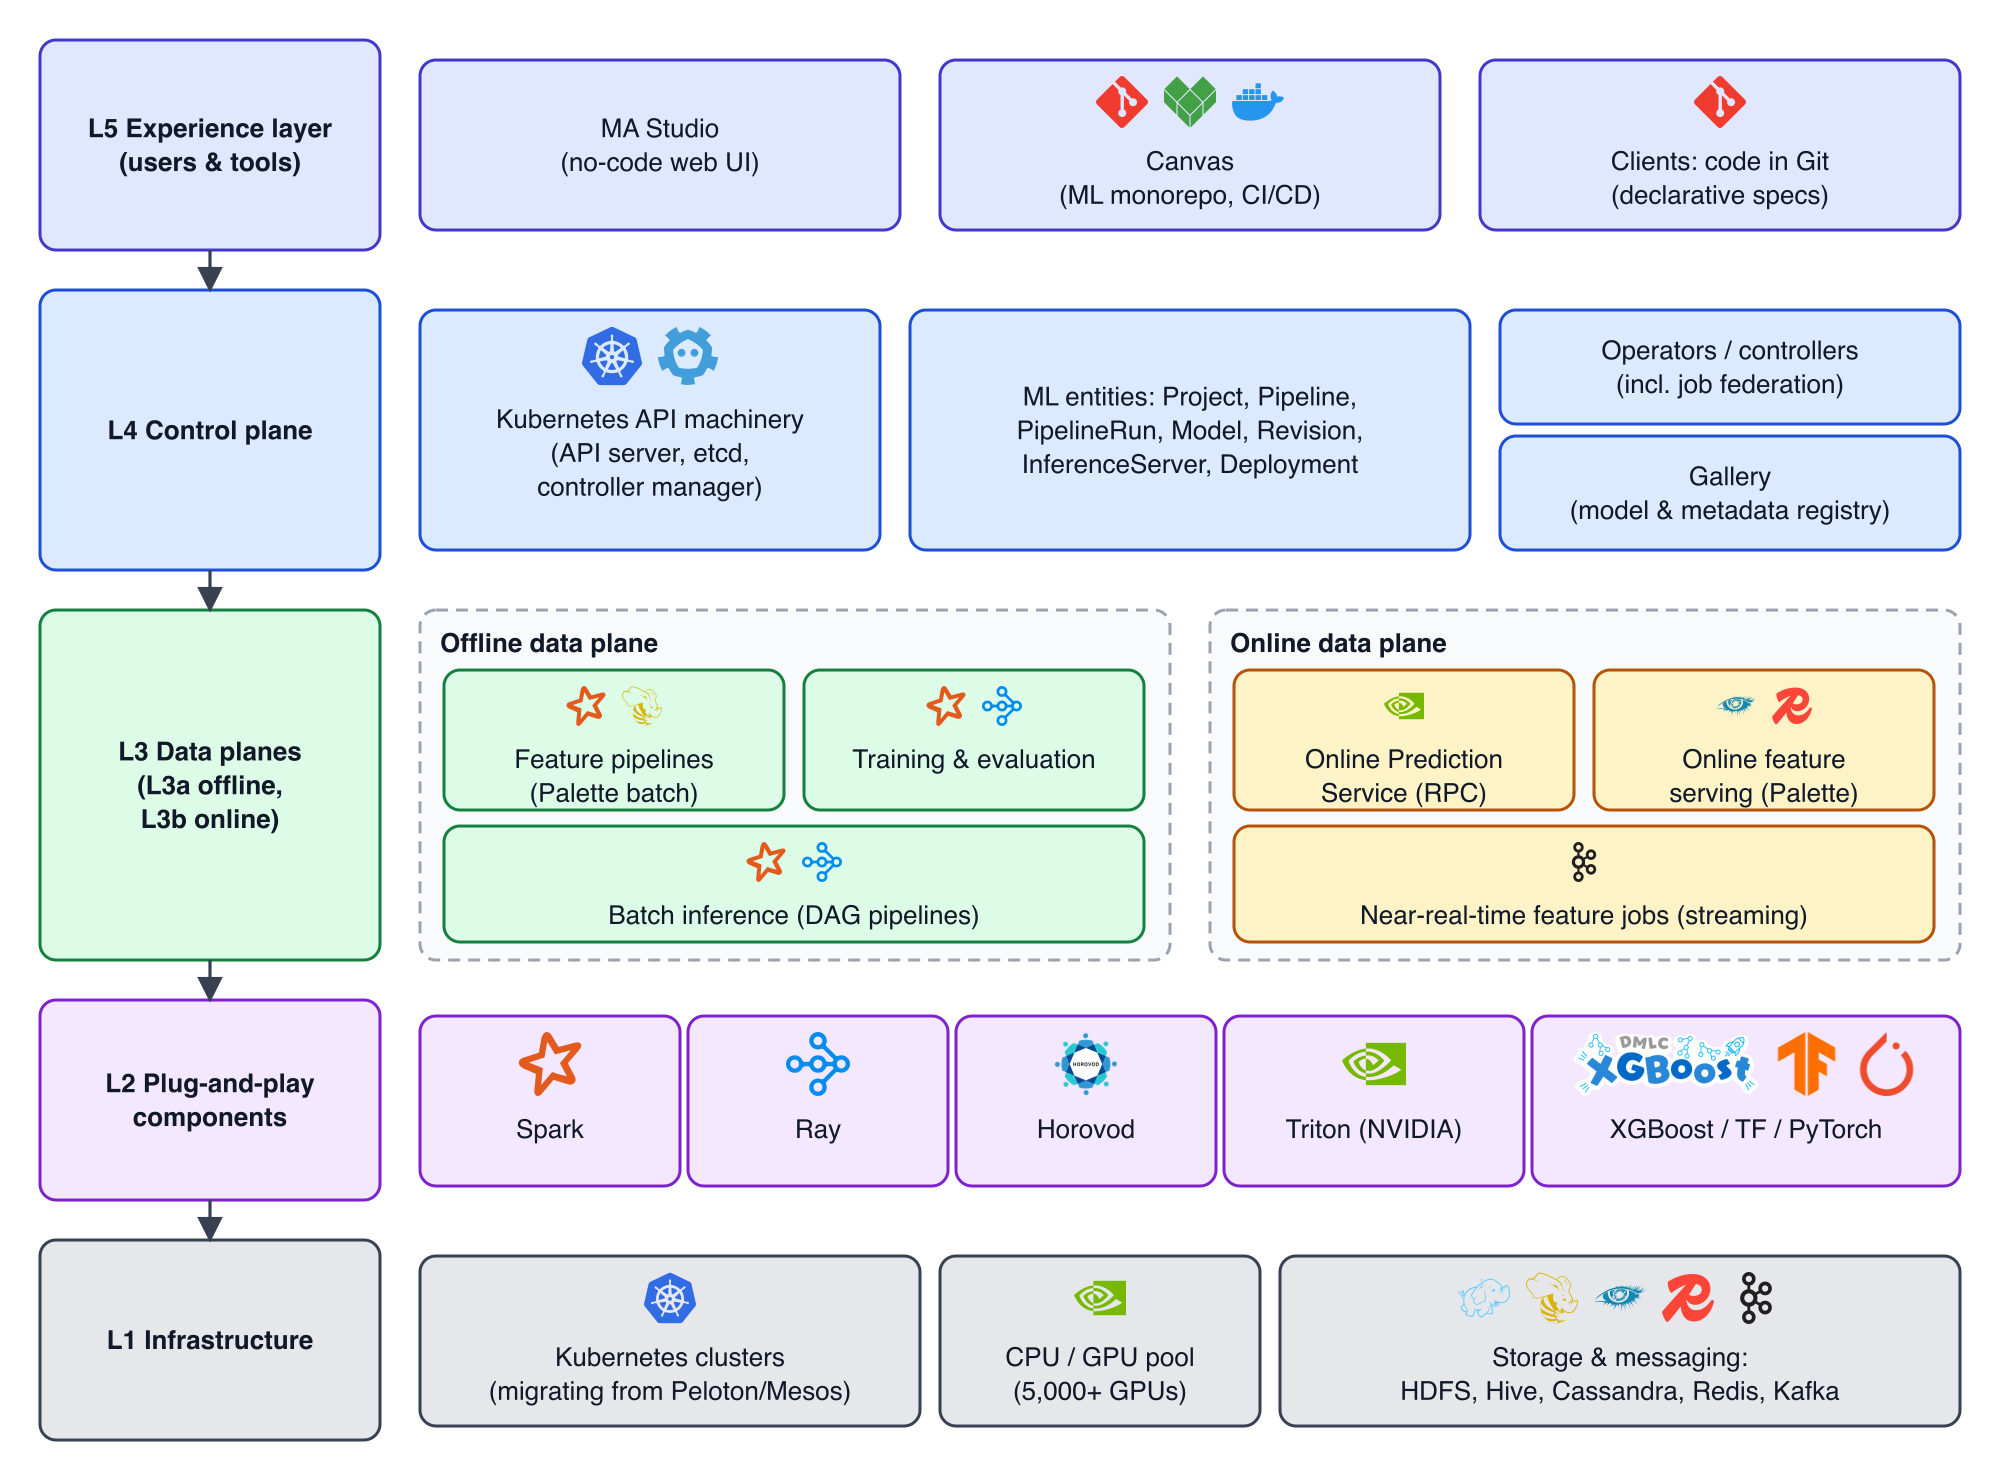
\includegraphics[width=\linewidth]{memberD-fig5-1-layered-view}
  \caption[Layered view of Michelangelo 2.0]{Layered view of Michelangelo 2.0.
    Each arrow means ``uses'' (top-down only). The offline and online data
    planes are peers inside layer L3.}
  \label{fig:layered-view}
\end{figure}

\begin{table}[ht]
  \centering
  \small
  \caption{Responsibilities, components and technologies of each layer.}
  \label{tab:layers}
  \begin{tabularx}{\linewidth}{@{}L{2.3cm}*{3}{>{\raggedright\arraybackslash}X}@{}}
    \toprule
    \textbf{Layer} & \textbf{Responsibility} & \textbf{Main components} & \textbf{Technologies} \\
    \midrule
    L5 Experience & Define and inspect ML work
      & MA Studio (no-code UI), Canvas (ML monorepo, CI/CD)
      & Web UI, Git, Bazel, Docker~\cite{uber2024} \\
    L4 Control plane & User-facing APIs; lifecycle of all ML entities
      & API server, controllers, job federation, Gallery
      & Kubernetes API server, etcd, controller manager~\cite{uber2024} \\
    L3a Offline data plane & Features, training, evaluation, batch inference
      & Palette batch pipelines, training pipelines, batch scoring
      & Spark, Ray~\cite{uber2024}; Hive/HDFS~\cite{uber2017} \\
    L3b Online data plane & Real-time inference and feature serving
      & Online prediction service, online feature serving, streaming feature jobs
      & Triton~\cite{uber2024}; Cassandra/Redis~\cite{uber2024palette};
        Kafka, Samza~\cite{uber2017} \\
    L2 Plug-and-play & Swappable engines
      & Compute and serving engines, ML frameworks
      & Spark, Ray, Horovod, Triton, XGBoost, TensorFlow,
        PyTorch~\cite{uber2024} \\
    L1 Infrastructure & Compute, storage, messaging
      & Clusters, CPU/GPU pool, storage
      & Kubernetes (from Peloton/Mesos), 5,000+ GPUs~\cite{uber2024};
        HDFS, Cassandra, Kafka~\cite{uber2017} \\
    \bottomrule
  \end{tabularx}
\end{table}

\paragraph{Control plane (L4).}
\begin{itemize}
  \item It ``defines user-facing APIs and manages the lifecycle of all entities
        in the system''~\cite{uber2024}.
  \item It follows the Kubernetes Operator pattern and Kubernetes API
        conventions, using the API server, etcd and controller
        manager~\cite{uber2024}.
  \item Its standard ML entities are Project, Pipeline, PipelineRun, Model,
        Revision, InferenceServer and Deployment~\cite{uber2024}. \emph{Our
        interpretation:} given the Kubernetes conventions and the named ``job
        CRD controller''~\cite{uber2024}, they are likely Kubernetes custom
        resources, as Palette's Feature and FeatureStore
        are~\cite{uber2024palette}.
  \item The API is \emph{declarative}: users state the desired result, and
        controllers make reality match it. Changes can come from the UI or from
        code in Git~\cite{uber2024}.
  \item The \emph{job federation} controller spreads Spark and Ray jobs across
        clusters, hiding ``the region, and zone and cluster
        details''~\cite{uber2024}.
  \item Gallery is the model and metadata registry~\cite{uber2024}. It continues
        1.0's versioned model repository, which stored each model's
        configuration, metrics and parameters~\cite{uber2017}.
\end{itemize}

\paragraph{Offline data plane (L3a).}
\begin{itemize}
  \item It ``does the heavy lifting on big data processing'': features,
        training, evaluation and batch inference~\cite{uber2024}.
  \item Work runs as pipelines, which are DAGs of steps executed on Spark or
        Ray. Checkpoints let a pipeline resume without repeating finished
        steps~\cite{uber2024}.
  \item Palette supports batch feature pipelines~\cite{uber2024}, and offline
        features are kept as daily Hive snapshots~\cite{uber2024palette}.
\end{itemize}

\paragraph{Online data plane (L3b).}
\begin{itemize}
  \item It ``handles real-time model inference and feature serving'' for Uber's
        other microservices, through RPC services and streaming
        jobs~\cite{uber2024}.
  \item The Online Prediction Service (OPS) now uses Triton, which Uber
        describes as optimised for low-latency GPU serving~\cite{uber2024}.
  \item Online features live in Cassandra or Redis~\cite{uber2024palette}.
  \item In 2017, P95 latency was under 5\,ms for models without
        Cassandra-backed features and under 10\,ms with
        them~\cite{uber2017}. By 2024 the platform served 10 million
        predictions per second at peak~\cite{uber2024}.
\end{itemize}

% ------------------------------------------------------------
\subsection{Dependencies and Communication Between Layers}
\label{sec:layered-communication}

Dependencies point strictly \textbf{top-down}: upper layers command lower ones,
and lower layers never call upward. Information returns upward only in two ways:
\begin{itemize}
  \item as \textbf{status} written back to control-plane resources (Kubernetes
        convention~\cite{uber2024});
  \item as \textbf{data} left in shared storage.
\end{itemize}
\Cref{fig:layered-communication} traces the main interactions.

\begin{figure}[ht]
  \centering
  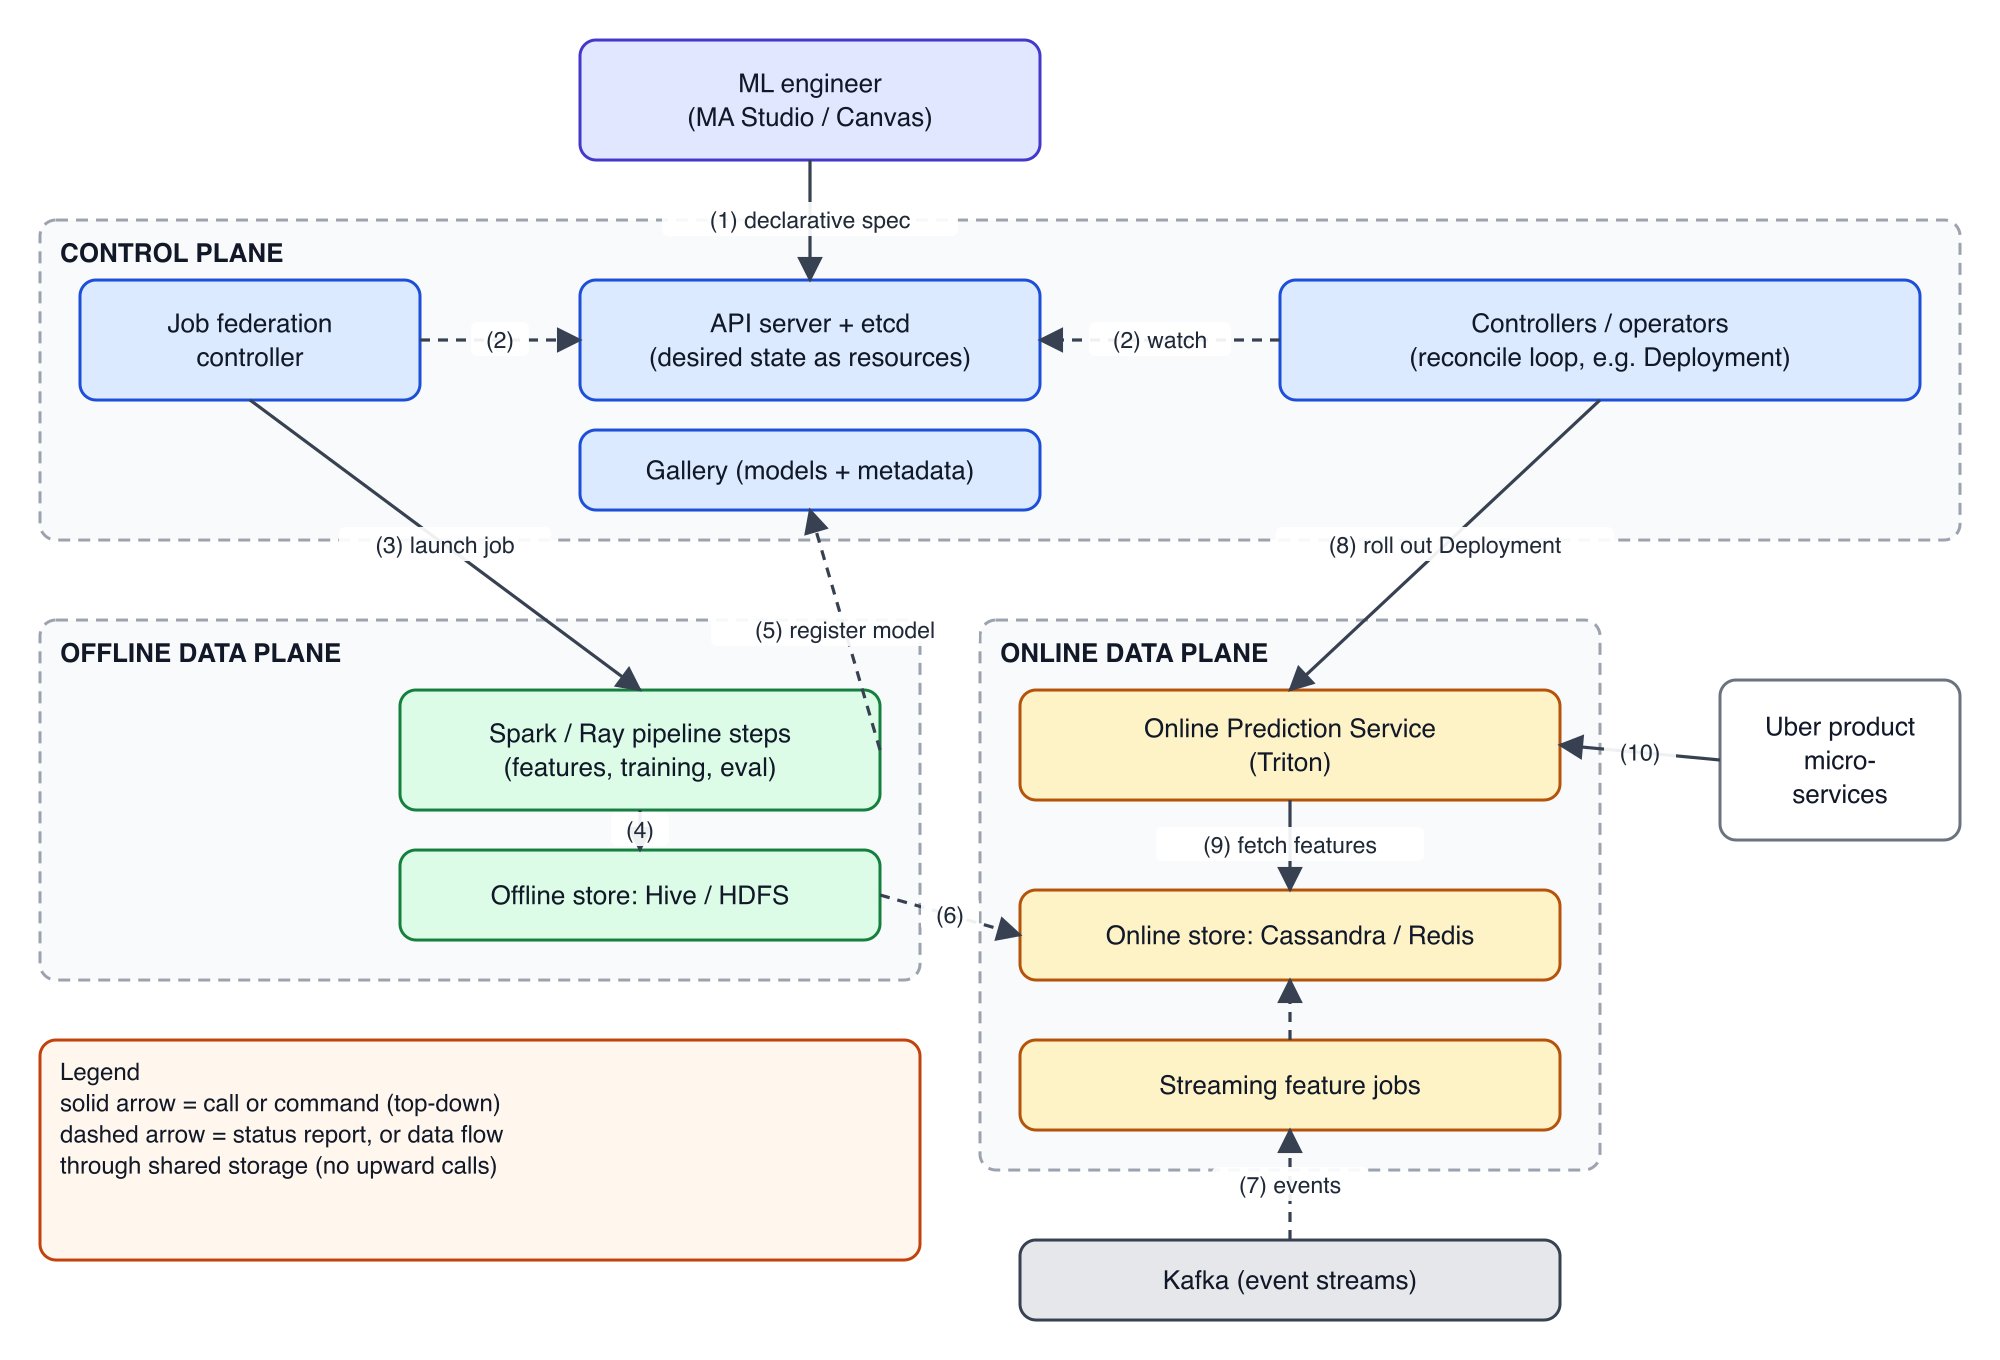
\includegraphics[width=\linewidth]{memberD-fig5-2-communication}
  \caption[Dependencies and communication between the layers]{Dependencies and
    communication between the layers. Solid arrows are calls or commands;
    dashed arrows are status reports or data handed over through storage.}
  \label{fig:layered-communication}
\end{figure}

\begin{enumerate}
  \item An ML engineer submits a desired state (e.g.\ a Pipeline or Deployment)
        from MA Studio or Canvas~\cite{uber2024}.
  \item Controllers watch the API server, act to close the gap between desired
        and actual state, and report status~\cite{uber2024}.
  \item The job federation controller launches Spark or Ray jobs on any
        suitable cluster~\cite{uber2024}.
  \item Pipeline steps read the data lake and write features to the offline
        store~\cite{uber2017}.
  \item Training stores the model, its configuration and metrics as a new
        version in the model repository, which is Gallery in
        2.0~\cite{uber2017,uber2024}. This is a write into a shared store
        (Cassandra in 2017), not a call to the control plane's logic.
  \item \emph{Batch path:} historical features are loaded from HDFS into
        Cassandra~\cite{uber2017}.
  \item \emph{Speed path:} streaming jobs aggregate Kafka events into
        Cassandra~\cite{uber2017}.
  \item A controller rolls the model out to OPS, with ``safe and incremental
        zonal rollout'' and automatic rollback~\cite{uber2024}. Models are
        referenced by ID or tag, enabling side-by-side versions and A/B
        tests~\cite{uber2017}.
  \item At prediction time, the model's features are read from
        Cassandra~\cite{uber2017}.
  \item Uber's product microservices call the prediction service over
        RPC~\cite{uber2017,uber2024}.
\end{enumerate}

Two observations follow:
\begin{itemize}
  \item \textbf{The two data planes never call each other.} They share data
        through storage (steps 6--7) and are coordinated from above (steps 3
        and 8), so the online plane is independent of batch jobs.
  \item \textbf{Closed and open layers.} The control plane is \emph{closed}:
        every change goes through its declarative API. The plug-and-play layer
        is partly \emph{open}: the managed solution supports a curated subset,
        but advanced users can ``bring your own components''~\cite{uber2024}.
\end{itemize}

% ------------------------------------------------------------
\subsection{Other Architecture Styles Inside the Layers}
\label{sec:layered-other-styles}

Layering is Michelangelo's backbone, but each layer uses the style that fits its
job (\Cref{fig:layered-styles}).

\begin{figure}[ht]
  \centering
  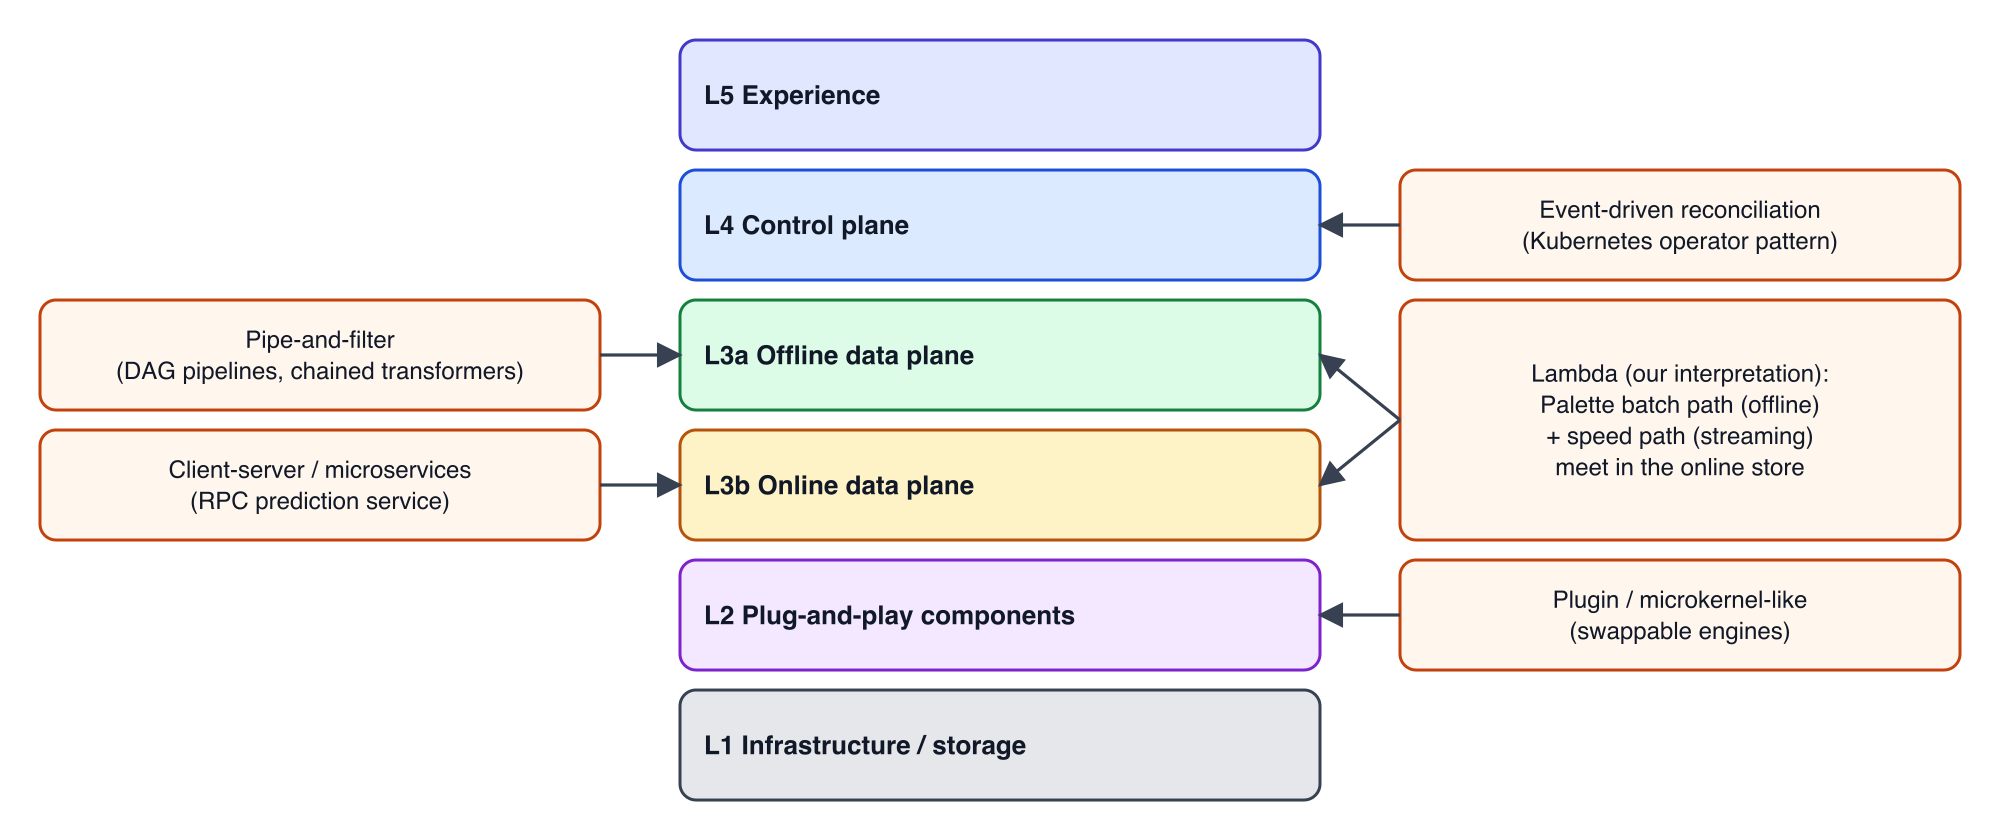
\includegraphics[width=\linewidth]{memberD-fig5-3-styles-in-layers}
  \caption[Other architecture styles placed in the layers]{Other architecture
    styles placed in the layers.}
  \label{fig:layered-styles}
\end{figure}

\begin{itemize}
  \item \textbf{Pipe-and-filter: offline data plane.} Pipelines are DAGs of
        steps, each consuming earlier outputs~\cite{uber2024}. Feature
        transformers are chained before the model, and Triton joined OPS as
        ``a new Spark transformer''~\cite{uber2024}.
  \item \textbf{Lambda: Palette, spanning both data planes} (\emph{our
        interpretation}). Batch and speed paths meet in a single serving
        store, Cassandra~\cite{uber2017}. This matches Lambda's batch, speed
        and serving layers, although Uber never uses the term.
  \item \textbf{Event-driven reconciliation: control plane.} Following the
        Kubernetes Operator pattern, controllers react to resource
        changes~\cite{uber2024}.
  \item \textbf{Plugin (microkernel-like): plug-and-play layer.}
        Plug-and-play is one of Uber's six design principles. Stable
        entities hide interchangeable engines~\cite{uber2024}.
  \item \textbf{Client-server / microservices: online data plane.} The
        prediction service answers RPC calls from other Uber
        services~\cite{uber2017}.
\end{itemize}

Layering decides \emph{what may depend on what}; each layer picks the style that
serves its own goal.

% ------------------------------------------------------------
\subsection{Evaluation: How Well Does Layering Serve Michelangelo?}
\label{sec:layered-evaluation}

\subsubsection{Benefits}

\paragraph{Benefit 1. Lower layers change without disturbing upper layers.}
Uber is migrating its clusters from Peloton/Mesos to Kubernetes and extending to
cloud GPUs on OCI and GCP~\cite{uber2024}. The job federation layer hides
cluster details for ``job portability''~\cite{uber2024}, so engineers keep
submitting the same pipelines while the infrastructure underneath changes. This
is the isolation the style promises~\cite{richards2020}.

\paragraph{Benefit 2. Engines are swapped inside a layer.}
\begin{itemize}
  \item Neuropod ``lacks continuous community support and is being
        deprecated'', so Triton replaced it in OPS~\cite{uber2024}.
  \item Uber ``replaced Spark-based XGBoost and DL trainers with Ray-based
        trainers \ldots{} for better scalability and reliability''. The earlier
        Horovod-on-Spark setup had ``introduced many operational
        complexities''~\cite{uber2024}. Horovod itself remains the distributed
        training framework~\cite{uber2024}.
  \item \emph{Our interpretation:} teams describe \emph{what} to train and
        deploy (Pipeline, Model, Deployment), not \emph{which engine} runs it,
        so these swaps stayed inside the lower layers.
\end{itemize}

\paragraph{Benefit 3. Reuse at scale.}
The 2018 infrastructure layer let teams build specialised platforms on
it~\cite{uber2018}. By 2024 one platform carried about 400 projects, 20,000+
training jobs per month and 5,000+ production models~\cite{uber2024}.

\subsubsection{Limitations}

\paragraph{Limitation 1. A fault in a shared lower layer spreads upward.}
\begin{itemize}
  \item \emph{What happened:} in 2021, a bad Palette metadata change stopped
        online serving from loading metadata at boot, breaking major Tier-1 use
        cases~\cite{uber2024palette}.
  \item \emph{Why:} schema validation ran client-side, so users on outdated
        code merged incorrect metadata. With no incremental update system,
        changing one feature group triggered updates to hundreds of
        them~\cite{uber2024palette}.
  \item \emph{Fix:} server-side validation, Feature and FeatureStore CRDs, a
        Kubernetes-based controller and delta propagation. End-to-end updates
        dropped from ``over an hour'' to about 15
        minutes~\cite{uber2024palette}.
  \item \emph{Our interpretation:} this is the classic layering risk. A layer
        that many others depend on needs stronger safeguards than any single
        caller.
\end{itemize}

\paragraph{Limitation 2. Extra hops cost latency} (\emph{our interpretation} of
Uber's data). Models that read features from the Cassandra storage layer had a
P95 target of under 10\,ms, against under 5\,ms for models that did
not~\cite{uber2017}. Every hop into a lower layer on the request path consumes
latency budget.

\paragraph{Limitation 3. Rigidity and cross-layer change.}
\begin{itemize}
  \item Michelangelo 1.0's config- and UI-driven path slowed iteration. Uber's
        lesson was ``let developers use the tools that they want'', which led
        it to add PyML~\cite{uber2018}.
  \item The Spark-based feature transformation DSL could not run on GPUs, which
        limited low-latency deep-learning serving~\cite{uber2024}. A concern
        shared by several layers needs coordinated change across all of them.
  \item Uber's answer was to open layers selectively (Canvas, ``bring your own
        components'')~\cite{uber2024}.
\end{itemize}

\subsubsection{Overall assessment}
Layering isolates fast-changing infrastructure and engines from hundreds of
product teams and lets one platform be shared at scale. Its costs are the
classic ones: fragile shared layers, latency per hop and rigidity. Uber kept the
layers and managed these costs with stronger validation in shared layers, a
separate online plane and deliberately opened layers. \emph{Our
interpretation:} the move from the loosely layered 1.0 to the explicit
three-plane 2.0 suggests that a large MLOps platform benefits from \emph{more}
layering discipline over time, not less.
  % Member F
% sections/06-conclusion.tex
% OWNER: Member A (Nhom truong)
% Do NOT edit this file if you are not Member A.

\section{Conclusion}
\label{sec:conclusion}

\subsection{Summary of Findings}
% [Member A] Recap the main points of the report in 3-5 sentences.

This report has presented a layered MLOps architecture that separates data
engineering, model training, model governance, and production serving into four
distinct layers with well-defined contracts.
The layered model satisfies the primary architectural drivers---reproducibility,
scalability, and reliability---while remaining feasible for a seven-person team.
The principal trade-off is increased operational complexity, which is mitigated
through managed cloud services and infrastructure automation.

\subsection{Lessons Learned}
% [Member A] Reflect on what worked and what would be done differently.

\begin{itemize}
  \item The feature store significantly reduced training-serving skew and
        should be introduced early, not added as an afterthought.
  \item Event-driven retraining requires careful schema governance on the drift
        event contract to avoid silent failures.
  \item Separating the serving cluster from the training cluster was the single
        most effective decision for meeting the latency constraint.
\end{itemize}

\subsection{Future Work}
% [Member A] List extensions or improvements for future milestones.

\begin{enumerate}
  \item Introduce per-module database isolation as traffic grows.
  \item Evaluate federated learning for privacy-sensitive datasets.
  \item Automate the model-approval workflow with a shadow-mode evaluation
        harness.
  \item Extend monitoring to cover fairness and bias metrics.
\end{enumerate}
            % Member A (nhom truong)

% ============================================================
%  Bibliography
% ============================================================
\bibliographystyle{plainnat}
\bibliography{references}

\end{document}
